\section{Relevancia del proyecto}

\begin{frame}
    \frametitle{Escasez de agua}
    
    \begin{columns}
        \begin{column}{0.5\textwidth}
        		\Large\bfseries\centering \acrshort{pnud}
        \end{column}
        \begin{column}{0.5\textwidth}
        		\Large\bfseries\centering \acrshort{wri}
        \end{column}
    \end{columns}
    
    \vspace*{5mm}
    
    \begin{columns}
        \begin{column}{0.5\textwidth}
	        	\centering
        		2022: Afecta a +\qty{40}{\percent} de la población mundial
        \end{column}
        \begin{column}{0.5\textwidth}
        		\centering
        		2025: 3500 millones de personas en regiones de escasez
        \end{column}
    \end{columns}
    
    \vspace*{5mm}
    
    \begin{columns}
        \begin{column}{0.25\textwidth}
            \centering
            \begin{figure}
                \centering
                
\includegraphics[
                    height=35mm,
                    width=\linewidth,
                    keepaspectratio
                ]{Relevancia/enfermedades.png}
                \caption{Enfermedades}
            \end{figure}
        \end{column}			
        \begin{column}{0.25\textwidth}
            \centering
            \begin{figure}
                \centering
                
\includegraphics[
                    height=35mm,
                    width=\linewidth,
                    keepaspectratio
                ]{Relevancia/ecosistemas.png}
                \caption{Pérdida de biodiversidad}
            \end{figure}
        \end{column}
        \begin{column}{0.25\textwidth}
            \centering
            \begin{figure}
                \centering
                
\includegraphics[
                    height=35mm,
                    width=\linewidth,
                    keepaspectratio
                ]{Relevancia/industrias.png}
                \caption{Afectaciones a industrias}
            \end{figure}
        \end{column}
        \begin{column}{0.25\textwidth}
            \centering
            \begin{figure}
                \centering
                
\includegraphics[
                    height=35mm,
                    width=\linewidth,
                    keepaspectratio
                ]{Relevancia/conflictos.png}
                \caption{Conflictos sociales}
            \end{figure}
        \end{column}
    \end{columns}
\end{frame}

\begin{frame}
    \frametitle{Planteamiento del problema}
    \begin{displayquote}
        \justifying
        \textbf{ODS 6.a.} De aquí a 2030, ampliar la cooperación internacional y el apoyo prestado a los países en desarrollo para la creación de capacidad en actividades y programas relativos al agua y el saneamiento, como los de captación de agua, \textbf{\gls{desalinizacion}}, uso eficiente de los recursos hídricos, tratamiento de aguas residuales, reciclado y tecnologías de reutilización \cite{naciones_unidas_sustainable_nodate}.
    \end{displayquote}\vspace*{6mm}
    \centering
    \begin{figure}
        \centering
        
\includegraphics[height=35mm, keepaspectratio]{ONU.png}
        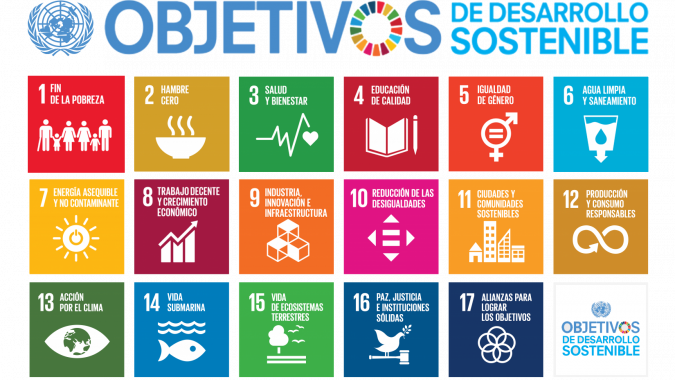
\includegraphics[height=35mm, keepaspectratio]{ods.png}
        \caption{Objetivos de desarrollo sostenible}
    \end{figure}
    
\end{frame}